\chapter{Performance analysis}
\section{Testing aparatus}
Some of the results in this section was generated using one node of the UCT ICTS High Performance HEX cluster, which has 4 16-core AMD Opteron 6376 CPUs. The CPUs
have have a maximum memory bandwidth of 51.2 GB/s \footnote{According to AMD, \url{http://www.amd.com/en-us/products/server/opteron/6000/6300\#}}

The GPU results were generated on a machine with 4 8-core Intel Xeon E5-2690 with 1 NVIDIA Tesla K40m co-processor (compute capability 3.5) at Rhodes University. The K40m has a maximum
memory bandwidth of 288 GB/s \footnote{According to the Nvidia Tesla-Kepler Family Datasheet}. The Nvidia CUDA toolkit version 6.5 was used to compile our imager. 
\section{Metrics}
The primary performance metric used to measure gridder performance was Giga Grid Point Additions per second (abbriviated ``G''). This metric includes the size of the
convolution filter support, number of correlations and number of channels being gridded per dataset record:
\begin{equation}
 \text{Giga grid point additions per second} := \frac{\tau_\text{observed}}{\tau_\text{integration}}N_\text{baselines}N_\text{channel}N_\text{corr}C_\text{sup}^210^{-9}s^{-1}
\end{equation}

In our discussion we include the time needed to copy visibilities onto the GPU and images back to the host in this calculation, but exclude fourier transform costs.
\section{Dataset simulation pipelines}
Three datasets were simulated for the experiments presented in this chapter. The datasets in measurement set format was generated using makems tool\footnote{Available at
\url{https://github.com/ska-sa/makems}}. Dataset 1 is generated using a benchmarking tool included with our imager. It should be noted that both EVLA and MeerKAT observations
have many more available channels than the number used; the Expanded Very Large Array has a minimum of 16384 spectral channels\cite{2041-8205-739-1-L1} for instance.

For each of the telescopes the approximate diffraction limited beam radius is shown, as well as the minimum Nyquest cell size and corresponding number of pixels. The experiments used grids padded
with enough pixels to account for the size of the convolution filter.
\begin{table}[ht]
  \centering
  \begin{tabular}[c]{|c||c|c|c|}
  \hline
  & (1) EVLA (small) & (2) EVLA (large) & (3) MeerKAT (large) \\
  \hline
  $\tau_\text{observed}$ & 4hrs & 4hrs &\\
  \hline
  $\tau_\text{integration}$ & 8.49056 & 3.00 &\\
  \hline
  $\nu_\text{min}$ & 1.2 GHz (L-band) & 1.2 GHz &\\
  \hline
  D & 25m & 25m &\\
  \hline
  B & 1km (D-conf) & 1km &\\
  \hline
  $N_\text{ant}$ & 27 & 27 &\\
  \hline
  $N_\text{bl}$ & 378 & 378 &\\
  \hline
  $N_\text{spw}$ & 1 & 1 &\\
  \hline
  $N_\text{chan}$ & 128 & 128 &\\
  \hline
  $N_\text{corr}$ & 1,2,4 & 4 &\\
  \hline
  Type & benchmark & ms &\\
  \hline
  Dataset size (vis only) & 313.03 MiB & 6.92 GiB &\\
  \hline
  Diffraction limited Image Radius & 34.35368 arcmins & 34.35368 arcmins &\\
  \hline
  Critical sampling cell size & 0.42942 arcmins & 0.42942 arcmins &\\
  \hline
  Minimum number of pixels & $80^2$ & $80^2$ &\\
  \hline
  \end{tabular}
  \caption[]{}
  \label{tbl_datasets}
\end{table}
\section{Scalability}
\subsection{Faceting only}
For the first experiment 144 facets are created on both the CPU and GPU. For this experiment w-projection is disabled and the convolution filter
(real) is limited to full support of 7 pixels. Only a single correlation of dataset 2 is gridded. Both single and double precision performance is indicated in
Figure~\ref{FIG_FACETING_CPU_VS_GPU}.
\begin{figure}[ht!]
 \begin{mdframed}
 \centering
 \begin{tikzpicture}
  \pgfplotstableread{ % Read the data into a table macro
    Cores	Single			Double
    1		0.168316854		0.1685377785
    2		0.3360213479		0.331968964
    4		0.6695498991		0.6697305849
    8		1.3327786378		1.3252101804
    12		1.9154355731		1.9005565542
    16		2.4924566532		2.4509550484
    32		2.9869489438		2.9737917788
    48		3.8490227827		3.7533815409
    64		3.9300946017		3.3901422435
    128		3.8010802609		3.4347945222
    GT770	3.3958577873		1.0339093049
    K40m	4.0599346466		1.9516763759
    c		0			0
  }\datatable

  \begin{axis}[
    legend style={at={(0.5,-0.20)}, anchor=north,legend columns=-1},
    ymin=0,         % Start y axis at 0
    xmin=1,
    xmax=c,
    symbolic x coords={1,2,4,8,12,16,32,48,64,128,GT770,K40m,c},
    xlabel=Threads/GPU,
    ylabel=Giga Grid Point Additions Per Second,
    grid=major,    
    visualization depends on=y \as \rawy,
    scale only axis, % The height and width argument only apply to the actual axis
    height=0.30\textheight,
    width=0.85\textwidth,
    minor y tick num=1,
    ybar interval=0.75
    ]
    \addplot table [x=Cores, y=Single] {\datatable};
    \addplot table [x=Cores, y=Double] {\datatable};
    \legend{Single Precision , Double Precision}
  \end{axis}
    
  \end{tikzpicture}
  \caption[]{}
  \label{FIG_FACETING_CPU_VS_GPU}
  \end{mdframed}
\end{figure}

Figure~\ref{FIG_FACETING_GPU} shows performance on the K40m GPU when the number of facets are varied. In each
case the total field of view was kept constant. W-projection is kept disabled. 
\begin{figure}[ht!]
 \begin{mdframed}
 \centering
 \begin{tikzpicture}
  \pgfplotstableread{ % Read the data into a table macro
    Facets	Single		Double
    1x1		1.9922928167	0.8772800235
    2x2		3.5881761479	1.4743756911
    3x3		3.9685656921	1.7718154723
    4x4		4.074639327	1.8163091046
    5x5		4.176103629	1.943378127
    6x6		4.2190583575	1.9588601963
    7x7		4.2536974869	1.9285941901
    8x8		4.2769083209	2.0129522373
    9x9		4.2859019484	1.9664906351
    10x10	4.2996766892	2.0451747578
  }\datatable

  \begin{axis}[
    legend style={at={(0.5,-0.20)}, anchor=north,legend columns=-1},
    symbolic x coords={1x1,2x2,3x3,4x4,5x5,6x6,7x7,8x8,9x9,10x10},
    ymin=0,         % Start y axis at 0
    xlabel=Number of facets,
    ylabel=Giga Grid Point Additions Per Second,
    grid=major,    
    visualization depends on=x \as \rawx,
    visualization depends on=y \as \rawy,
    scale only axis, % The height and width argument only apply to the actual axis
    height=0.25\textheight,
    width=0.85\textwidth,
    minor y tick num=1,
    nodes near coords,
    every node near coord/.append style={font=\tiny}
    ]
    \addplot table [x=Facets, y=Single] {\datatable};
    \addplot table [x=Facets, y=Double] {\datatable};
    \legend{Single Precision , Double Precision}
  \end{axis}
    
  \end{tikzpicture}
  \caption[]{}
  \label{FIG_FACETING_GPU}
  \end{mdframed}
\end{figure}

The next experiment used dataset 1 and was run using the Rhodes machine. It shows the dependance of gridding 
performance on the facet transforms. Again no w-projection was enabled, full support of 7 pixels was used and 
only a single facet is created. The results are shown in Figure~\ref{FIG_FACETING_SUPPORT_CPU}.
\begin{figure}[ht!]
 \begin{mdframed}
 \centering
 \begin{tikzpicture}
  \pgfplotstableread{ % Read the data into a table macro
    Support	Single		Double		Single_F	Double_F
    7		0.391535842	0.7802259806	0.3563959657	0.6578618005
    15		0.438040399	0.8477799805	0.4169094319	0.7989777737
    23		0.433364347	0.8942843078	0.4072700207	0.8765948472
    31		0.4426994228	0.9141481861	0.4190847247	0.9037965766
    63		0.4514632753	0.9120384589	0.4287080595	0.9147389089
    95		0.4563549187	0.9462958594	0.4392881355	0.9511770306
  }\datatable

  \begin{axis}[
    legend style={at={(0.5,-0.20)}, anchor=north,legend columns=-1},
    ymin=0,         % Start y axis at 0
    xlabel=Full support,
    ylabel=Giga Grid Point Additions Per Second,
    grid=major,    
    visualization depends on=x \as \rawx,
    visualization depends on=y \as \rawy,
    scale only axis, % The height and width argument only apply to the actual axis
    height=0.25\textheight,
    width=0.85\textwidth,
    minor y tick num=1,
    nodes near coords,
    every node near coord/.append style={font=\tiny}
    ]
    \addplot table [x=Support, y=Single] {\datatable};
    \addplot table [x=Support, y=Double] {\datatable};
    \addplot [every node near coord/.append style={shift={(0pt,-10pt)},font=\tiny}, mark=square*, color=black] table [x=Support, y=Single_F] {\datatable};
    \addplot [every node near coord/.append style={shift={(0pt,-10pt)},font=\tiny}, mark=triangle*, color=brown] table [x=Support, y=Double_F] {\datatable};
    \legend{SP, DP, SP (Faceting), DP (Faceting)}
  \end{axis}
    
  \end{tikzpicture}
  \caption[]{}
  \label{FIG_FACETING_SUPPORT_CPU}
  \end{mdframed}
\end{figure}

\subsection{W-projection scaling}
Figure~\ref{FIG_WPROJECTION_SUPPORT_SCALING_GPU} shows how w-projection scales with filter full support size on the K40m.
The performance for both real and complex (separable) filters are indicated. Here dataset 2 was used and faceting transforms
were disabled. Only a single correlation was gridded here.
\begin{figure}[ht!]
 \begin{mdframed}
 \centering
 \begin{tikzpicture}
  \pgfplotstableread{ % Read the data into a table macro
    Support	SP_Real		DP_Real		SP_W-projection		DP_W-projection
    7		1.5528886351	1.2956084019	1.5170246335		0.6890953378
    15		4.1295591352	2.7303211482	3.106550774		1.6977586185
    23		4.9051924869	3.150798132	3.7100625258		2.1236070793
    31		5.0391705103	3.3962147312	3.84011765		2.2470674278
    63		5.5095741708	3.6871730155	3.9305867278		2.2969014285
    95		5.6663495212	3.7558552376	3.9500724449		2.2786372089
    127		5.7419715351	3.7254606461	3.9268803718		2.2871868268
    255		5.8583062779	3.3745594577	3.4235019117		1.9973144153
  }\datatable

  \begin{axis}[
    legend style={at={(0.5,-0.20)}, anchor=north,legend columns=-1},
    ymin=0,         % Start y axis at 0
    xlabel=Full support,
    ylabel=Giga Grid Point Additions Per Second,
    grid=major,    
    visualization depends on=x \as \rawx,
    visualization depends on=y \as \rawy,
    scale only axis, % The height and width argument only apply to the actual axis
    height=0.25\textheight,
    width=0.85\textwidth,
    minor y tick num=1,
    nodes near coords,
    every node near coord/.append style={font=\tiny}
    ]
    \addplot [every node near coord/.append style={shift={(0pt,5pt)},font=\tiny}, mark=square*, color=red] table [x=Support, y=SP_Real] {\datatable};
    \addplot [every node near coord/.append style={shift={(0pt,-15pt)},font=\tiny}, mark=square*, color=blue] table [x=Support, y=DP_Real] {\datatable};
    \addplot [every node near coord/.append style={shift={(0pt,5pt)},font=\tiny}, mark=square*, color=black] table [x=Support, y=SP_W-projection] {\datatable};
    \addplot [every node near coord/.append style={shift={(0pt,-15pt)},font=\tiny}, mark=triangle*, color=brown] table [x=Support, y=DP_W-projection] {\datatable};
    \legend{SP (Real), DP (Real), SP (W-Projection), DP (W-Projection)}
  \end{axis}
  \end{tikzpicture}
  \caption[]{}
  \label{FIG_WPROJECTION_SUPPORT_SCALING_GPU}
  \end{mdframed}
\end{figure}

The CPU implementation uses vectorization when w-projection is enabled. Figure~\ref{FIG_WPROJECTION_AVX} shows the speedup between
AVX-vectorized gridding compared to a non-vectorized implementation gridding 1, 2 and 4 correlations.
\begin{figure}[ht!]
 \begin{mdframed}
 \centering
 \begin{tikzpicture}
  \pgfplotstableread{ % Read the data into a table macro
  Support	SP_1		DP_1		SP_2		DP_2		SP_4		DP_4
  7		1.0378929668	1.0450717281	1.2962282904	1.394842132	1.3058784272	1.3352135707
  15		1.3769345405	1.2246377124	1.742187934	1.8204448215	1.735783957	1.7707962707
  23		1.4363795888	1.4501275271	2.0014982329	2.0026917809	1.9637217201	1.973606804
  31		1.5002036529	1.493357172	2.1536070203	2.098407853	2.0879592035	2.0881374468
  63		1.6843553398	1.3603447834	2.4530139778	2.2203411915	2.3202820472	2.0267067347
  95		1.6832324591	1.3598832177	2.6108160929	2.2457821084	2.4224647411	1.756396849
  }\datatable

  \begin{axis}[
    legend style={at={(0.5,-0.20)}, anchor=north,legend columns=3},
    ymin=0,         % Start y axis at 0
    xlabel=Full support,
    ylabel=Speedup,
    grid=major,    
    visualization depends on=x \as \rawx,
    visualization depends on=y \as \rawy,
    scale only axis, % The height and width argument only apply to the actual axis
    height=0.25\textheight,
    width=0.85\textwidth,
    minor y tick num=1]
    \addplot table [x=Support, y=SP_1] {\datatable};
    \addplot table [x=Support, y=DP_1] {\datatable};
    \addplot table [x=Support, y=SP_2] {\datatable};
    \addplot table [x=Support, y=DP_2] {\datatable};
    \addplot table [x=Support, y=SP_4] {\datatable};
    \addplot table [x=Support, y=DP_4] {\datatable};
    \legend{SP (1-corr), DP (1-corr), SP (2-corr), DP (2-corr), SP (4-corr), DP (4-corr)}
  \end{axis}
  \end{tikzpicture}
  \caption[]{}
  \label{FIG_WPROJECTION_AVX}
  \end{mdframed}
\end{figure}

Figure~\ref{FIG_REAL_VS_WPROJ_CPU} shows the performance of w-projection (2D filter lookup table) with 
AVX enabled, as well as the performance of real-valued (separable 1D kernel) on the CPU, gridding dataset 1.
\begin{figure}[ht!]
 \begin{mdframed}
 \centering
 \begin{tikzpicture}
  \pgfplotstableread{ % Read the data into a table macro
  Support	SP_R		DP_R		SP_W		DP_W
  7		0.391535842	0.7802259806	0.3449583873	0.6981304878
  15		0.438040399	0.8477799805	0.5114612697	0.8516944559
  23		0.433364347	0.8942843078	0.5326320759	0.959799608
  31		0.4426994228	0.9141481861	0.5545785258	0.9957354413
  63		0.4514632753	0.9120384589	0.6274663523	0.8362027562
  95		0.4563549187	0.9462958594	0.597323049	0.8582801283
  }\datatable

  \begin{axis}[
    legend style={at={(0.5,-0.20)}, anchor=north,legend columns=-1},
    ymin=0,         % Start y axis at 0
    xlabel=Full support,
    ylabel=Giga Grid Point Additions Per Second,
    grid=major,    
    visualization depends on=x \as \rawx,
    visualization depends on=y \as \rawy,
    scale only axis, % The height and width argument only apply to the actual axis
    height=0.25\textheight,
    width=0.85\textwidth,
    nodes near coords,
    every node near coord/.append style={font=\tiny},
    minor y tick num=1]
    \addplot table [x=Support, y=SP_R] {\datatable};
    \addplot table [x=Support, y=DP_R] {\datatable};
    \addplot table [x=Support, y=SP_W] {\datatable};
    \addplot table [x=Support, y=DP_W] {\datatable};
    \legend{SP (Real), DP (Real), SP (W-projection), DP (W-projection)}
  \end{axis}
  \end{tikzpicture}
  \caption[]{}
  \label{FIG_REAL_VS_WPROJ_CPU}
  \end{mdframed}
\end{figure}
\subsection{W-faceting}
The next experiment shows scaling performance over filter support size for the K40m 
when faceting transforms are added to w-projection. Dataset 2 was used in generating
these results. Figure~\ref{FIG_FACET_VS_NO_FACET_GPU} shows the results of gridding in
single precision.
\begin{figure}[ht!]
 \begin{mdframed}
 \centering
 \begin{tikzpicture}
  \pgfplotstableread{ % Read the data into a table macro
  Support	No_Faceting	Faceting
  7		1.5170246335	1.569880153
  15		3.106550774	2.9654419599
  23		3.7100625258	3.4115842324
  31		3.84011765	3.521021361
  63		3.9305867278	3.6582319708
  95		3.9500724449	3.668447438
  127		3.9268803718	3.6621654057
  255		3.4235019117	3.2464487786
  }\datatable

  \begin{axis}[
    legend style={at={(0.5,-0.20)}, anchor=north,legend columns=-1},
    ymin=0,         % Start y axis at 0
    xlabel=Full support,
    ylabel=Giga Grid Point Additions Per Second,
    grid=major,    
    visualization depends on=x \as \rawx,
    visualization depends on=y \as \rawy,
    scale only axis, % The height and width argument only apply to the actual axis
    height=0.25\textheight,
    width=0.85\textwidth,
    nodes near coords,
    every node near coord/.append style={font=\tiny},
    minor y tick num=1]
    \addplot table [x=Support, y=No_Faceting] {\datatable};
    \addplot table [x=Support, y=Faceting] {\datatable};
    \legend{No Faceting (SP), Faceting (SP)}
  \end{axis}
  \end{tikzpicture}
  \caption[]{}
  \label{FIG_FACET_VS_NO_FACET_GPU}
  \end{mdframed}
\end{figure}
\section{Performance comparison against other imagers}
\subsection{Available software packages}
\subsection{Comparison}
\section{Discussion}
